%%%%%%%%%%%%%%%%%%%%%%%%%%%%%%%%%%%%%%%%%
% Stylish Title Page
% LaTeX Template
% Version 2.0 (22/7/17)
%
% This template was downloaded from:
% http://www.LaTeXTemplates.com
%
% Original author:
% Peter Wilson (herries.press@earthlink.net) with modifications by:
% Vel (vel@latextemplates.com)
%
% License:
% CC BY-NC-SA 3.0 (http://creativecommons.org/licenses/by-nc-sa/3.0/)
%
% This template can be used in one of two ways:
%
% 1) Content can be added at the end of this file just before the \end{document}
% to use this title page as the starting point for your document.
%
% 2) Alternatively, if you already have a document which you wish to add this
% title page to, copy everything between the \begin{document} and
% \end{document} and paste it where you would like the title page in your
% document. You will then need to insert the packages and document
% configurations into your document carefully making sure you are not loading
% the same package twice and that there are no clashes.
%
%%%%%%%%%%%%%%%%%%%%%%%%%%%%%%%%%%%%%%%%%

%----------------------------------------------------------------------------------------
%	PACKAGES AND OTHER DOCUMENT CONFIGURATIONS
%----------------------------------------------------------------------------------------

\documentclass[12pt]{article}
\usepackage[UKenglish]{babel}
\usepackage[margin=1in]{geometry}


\usepackage[utf8]{inputenc}
\usepackage[T1]{fontenc}
\usepackage{import}
\usepackage{lwworksheets}
\usepackage{graphicx}



\begin{document}

\frontpage{USB Macro Keypad}

%\import{../../worksheet-components}{title-page.tex}

\section{PCB}
\begin{instructions}
	\instruction{
		Read through \textit{all} these instructions thoroughly.
	}
	\instruction{
		Make the PCB (using the clear film artwork like in section
		\ref{sec:etch}.) with the help of a team member.  Be careful
		to clean up the edges of the board before exposing it. Ensure
		the artwork is the right way up on the light box.
	}
	\instruction{
		Drill \textbf{all} the holes with a 0.8mm drill bit.
	}
	\instruction{
		Looking carefully at the image in section \ref{sec:drillsizes},
		drill all the blue holes with a 1.5mm drill bit.
	}
	\instruction{
		Looking carefully at the image in section \ref{sec:drillsizes},
		drill all the red holes with a 1.75mm drill bit.
	}
	\instruction{
		Looking carefully at the image in section \ref{sec:drillsizes},
		drill all the purple holes with a 2.6mm drill bit.
	}
	\instruction{
		Looking carefully at the image in section \ref{sec:drillsizes},
		drill all the green holes with a 4mm drill bit.
	}
	\instruction{
		Ask a team member to check your PCB, then you can start
		soldering (section \ref{sec:soldering})
	}
\end{instructions}

\section{Soldering}
\label{sec:soldering}
\begin{instructions}
	\instruction{
		Check and identify all components. Attach these with masking
		tape to the sheet lablled "Parts List" (Section
		\ref{sec:partslist}).
	}
	\instruction{
		You are now going to solder the components to the board using
		the instructions below.  You will need to refer to Section
		\ref{sec:placement} to see where each component should go.
	}
	\instruction{
		Solder in the four \ohm{220} resistors, R1, R2, R3 and R4.
	}
	\instruction{
		Solder in the four \ohm{10k} resistors, R5, R6, R7 and R8.
	}
	\instruction{
		Solder in the two capacitors, C1 and C2, both 10nF.
	}
	\instruction{
		Insert the 4 transistors, Q1-4. \textbf{Do NOT} solder them yet,
		and be careful to insert them the right way round (see the
		picture in Section \ref{sec:placement}).
	}
	\instruction{
		Get a member of team to check the orientation of the
		transistors, then solder them in place.
	}
	\instruction{
		Insert the 4 LEDs, D1-4. \textbf{Do NOT} solder them yet, and be
		careful to insert them the right way round (see the picture in
		Section \ref{sec:placement}).
	}
	\instruction{
		Get a member of team to check the orientation of the
		LEDs, then solder them in place.
	}
	\instruction{
		Solder the 4-pin header in the holes for U2. The pins are close
		together, so be very careful not to bridge any pins when
		soldering.
	}
	\instruction{
		Ask a team member for the correct jig. Attach the two 20-pin
		headers to the jig and insert the headers into the board, then
		solder them in place. Again, be careful not to bridge any pins.
	}
	\instruction{
		Solder the switches SW1-9.
	}
	\instruction{
		Solder the rotary encoder SW10.
	}
	\instruction{
		Ask a member of team to check your soldering.
	}
\end{instructions}

\section{Final Assembly}
\begin{instructions}
	\instruction{
		Get a team member to check all your work.
	}
	\instruction{
		With a team member, insert the screen and the Pi Pico and attach
		a micro-USB cable to check that your project works correctly.
	}
	\instruction{
		Once it all works (and not before!), fit the key caps to the
		switches and the knob to the rotary encoder
	}
	\instruction{
		Fit four rubber feet to the four corners of the bottom of the
		PCB, and a fifth rubber foot directly underneath the rotary
		encoder.
	}
\end{instructions}

\section{Component Info}

%\explainLed
\begin{minipage}[t]{0.4\textwidth}
\begin{framed}
\subsection*{LED}
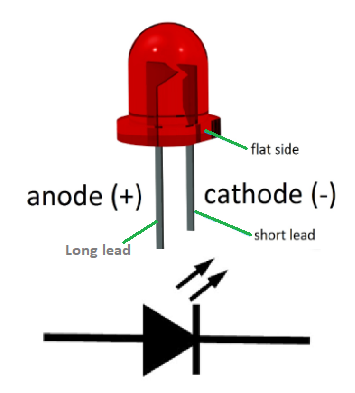
\includegraphics[width=\textwidth]{img/led-polarity.png}
\end{framed}
\end{minipage}

\explainMosfet

\section{Schematic}
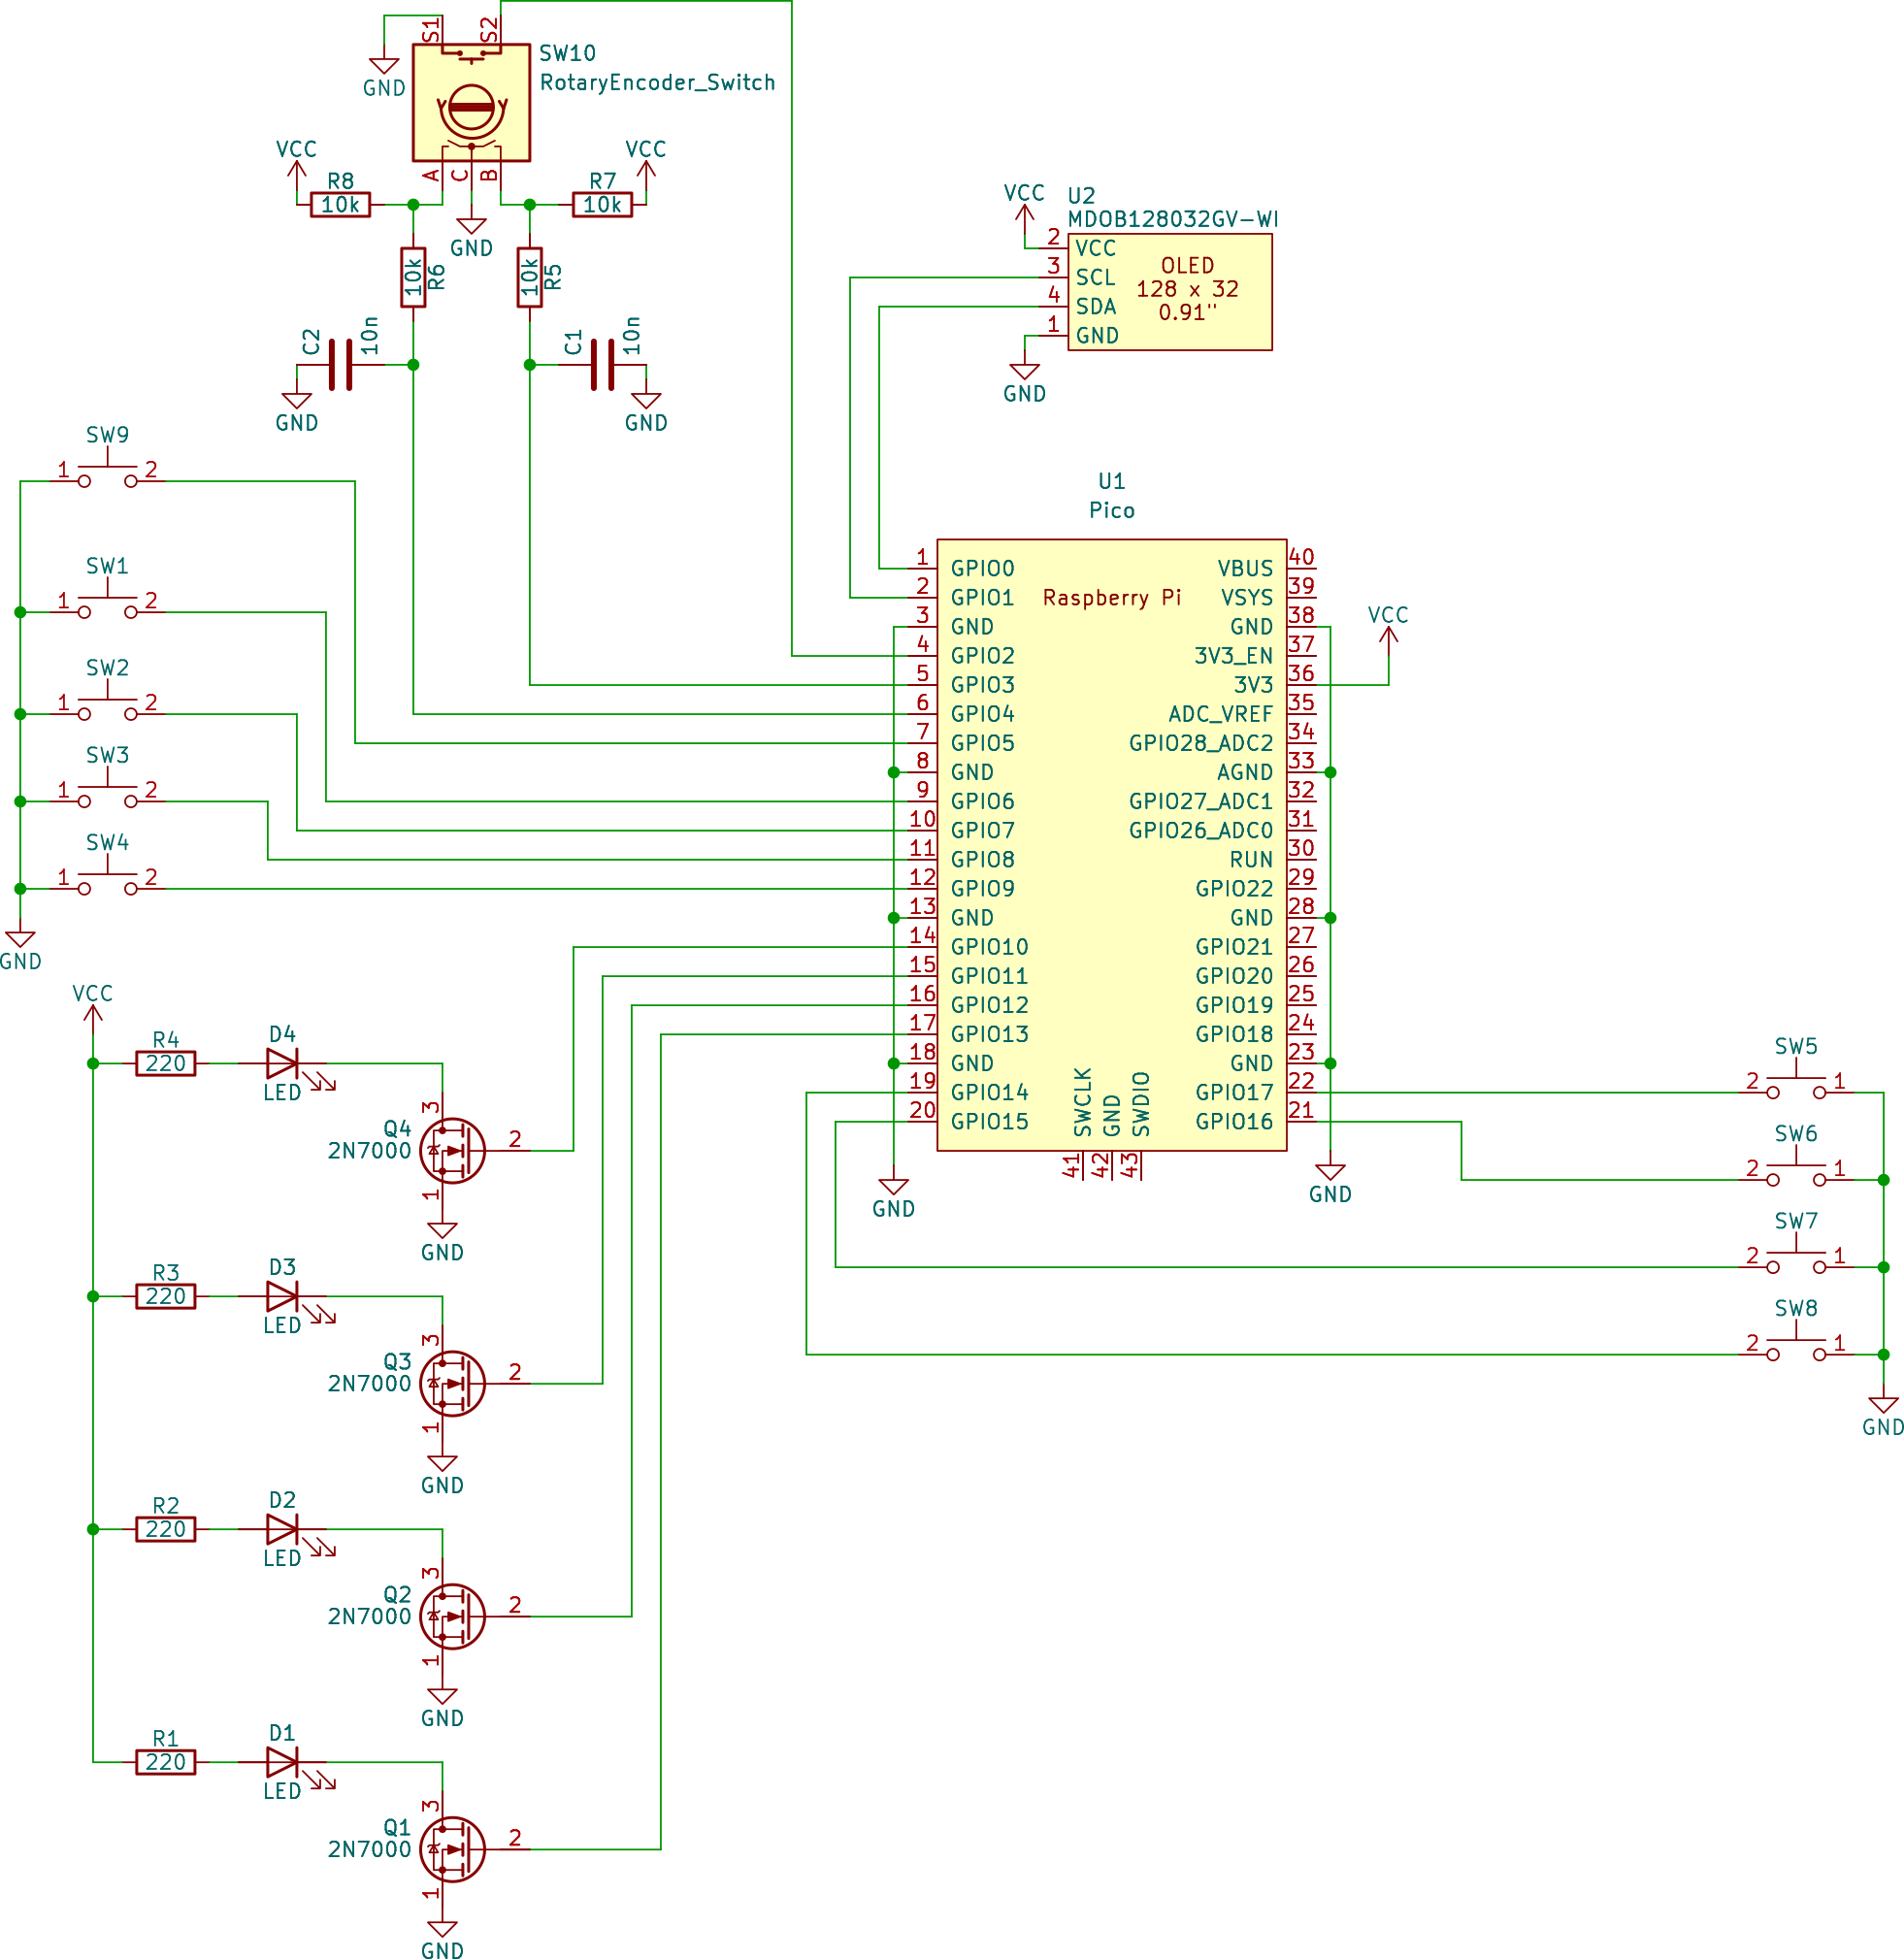
\includegraphics[width=\textwidth]{img/macropad-rev1-schematic.png}

\section{Etch}
\label{sec:etch}
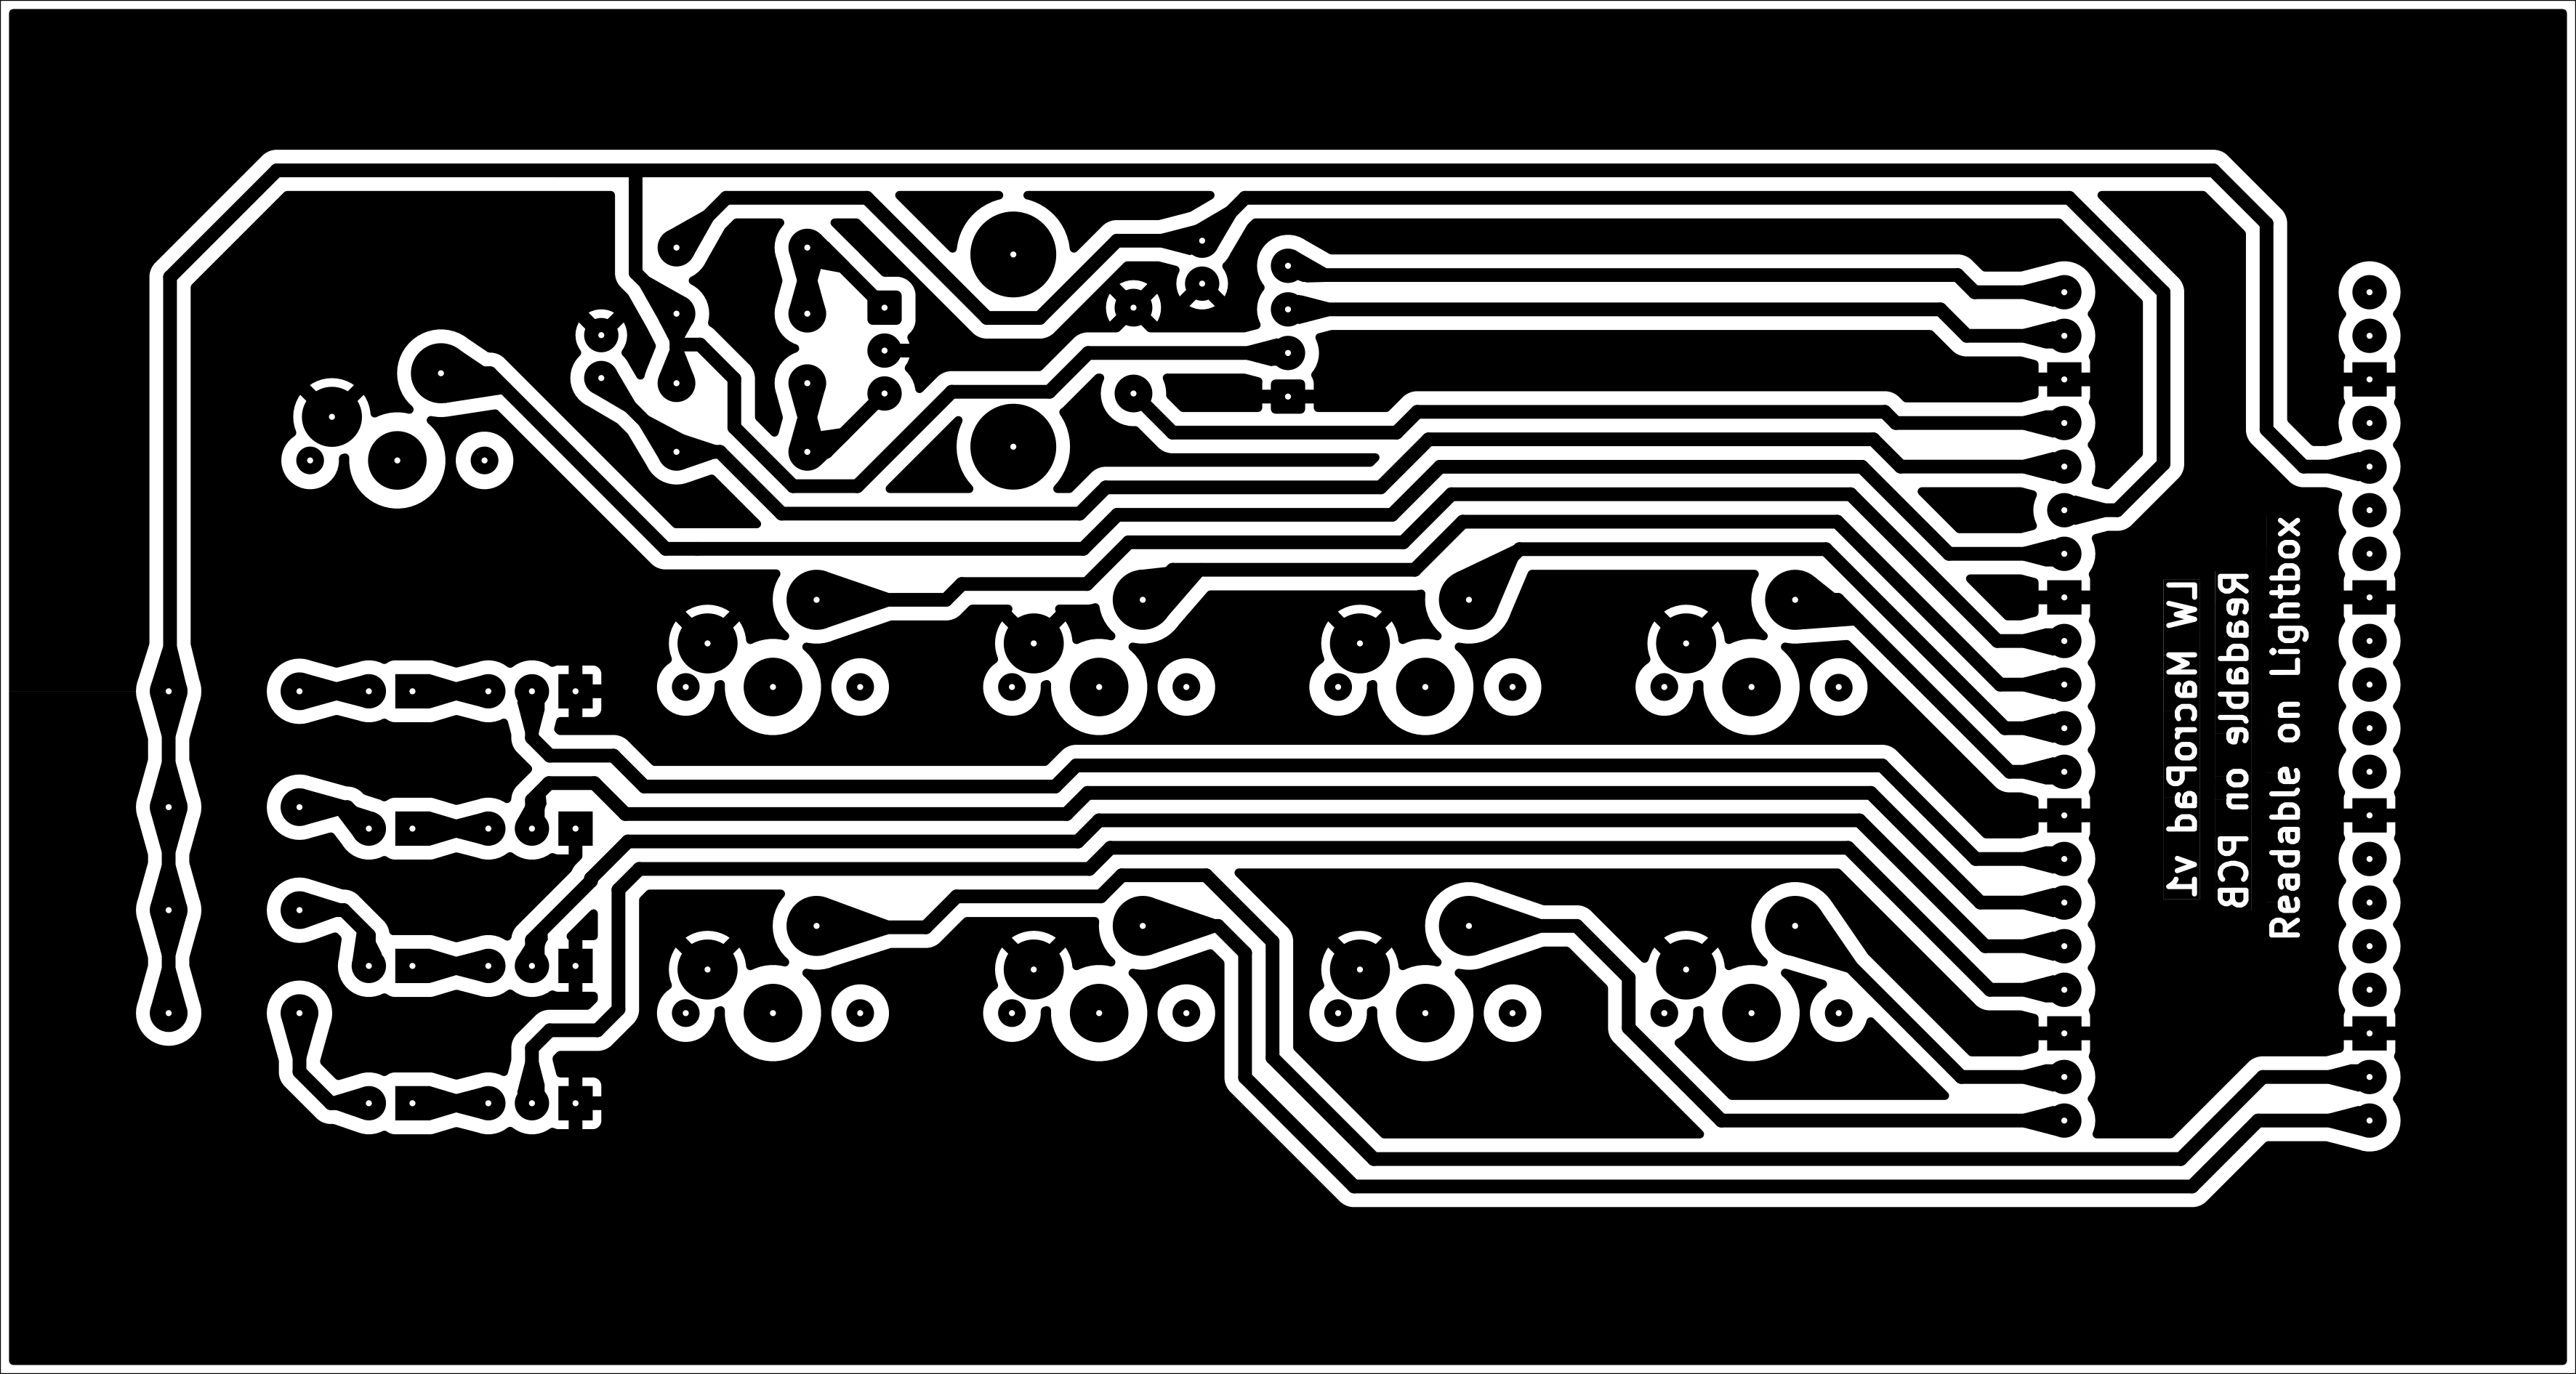
\includegraphics[width=\textwidth]{img/macropad-rev1-B_Cu_Oversized.png}

\section{Placement}
\label{sec:placement}
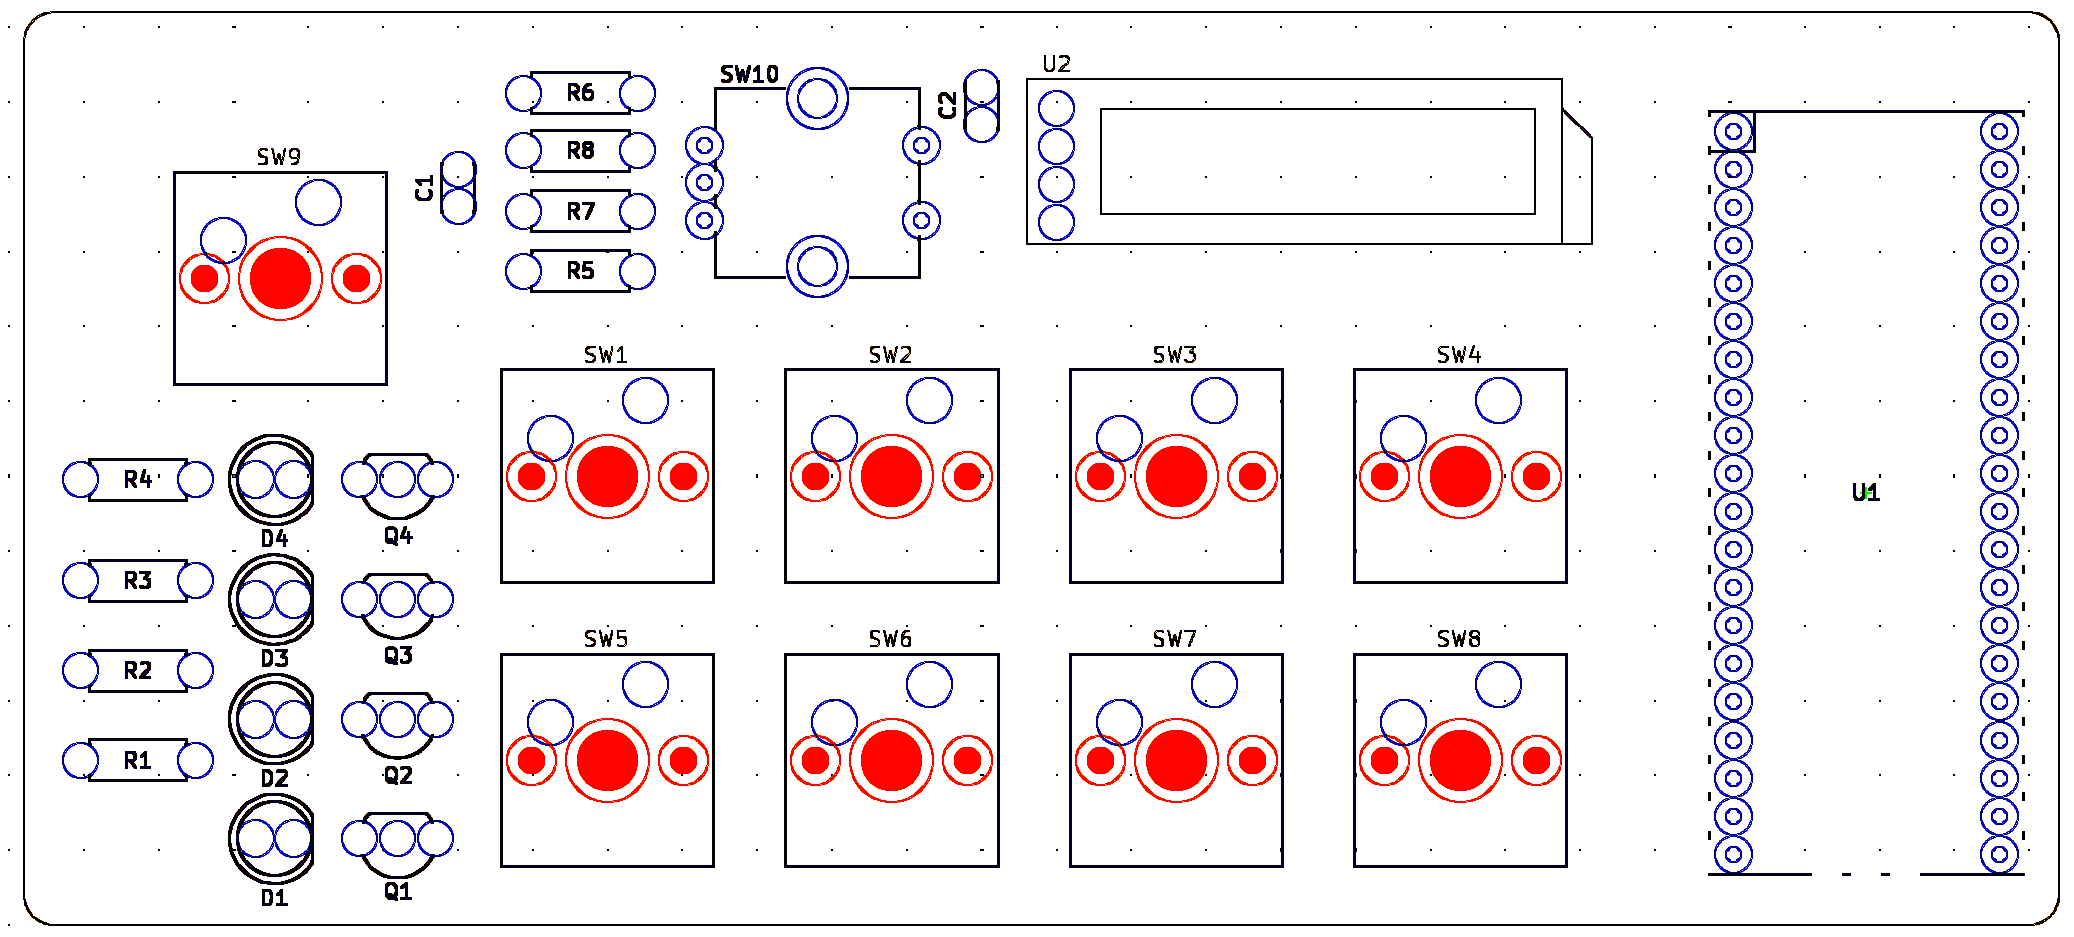
\includegraphics[width=\textwidth]{img/component-layout.png}


\section{Drill Sizes}
\label{sec:drillsizes}
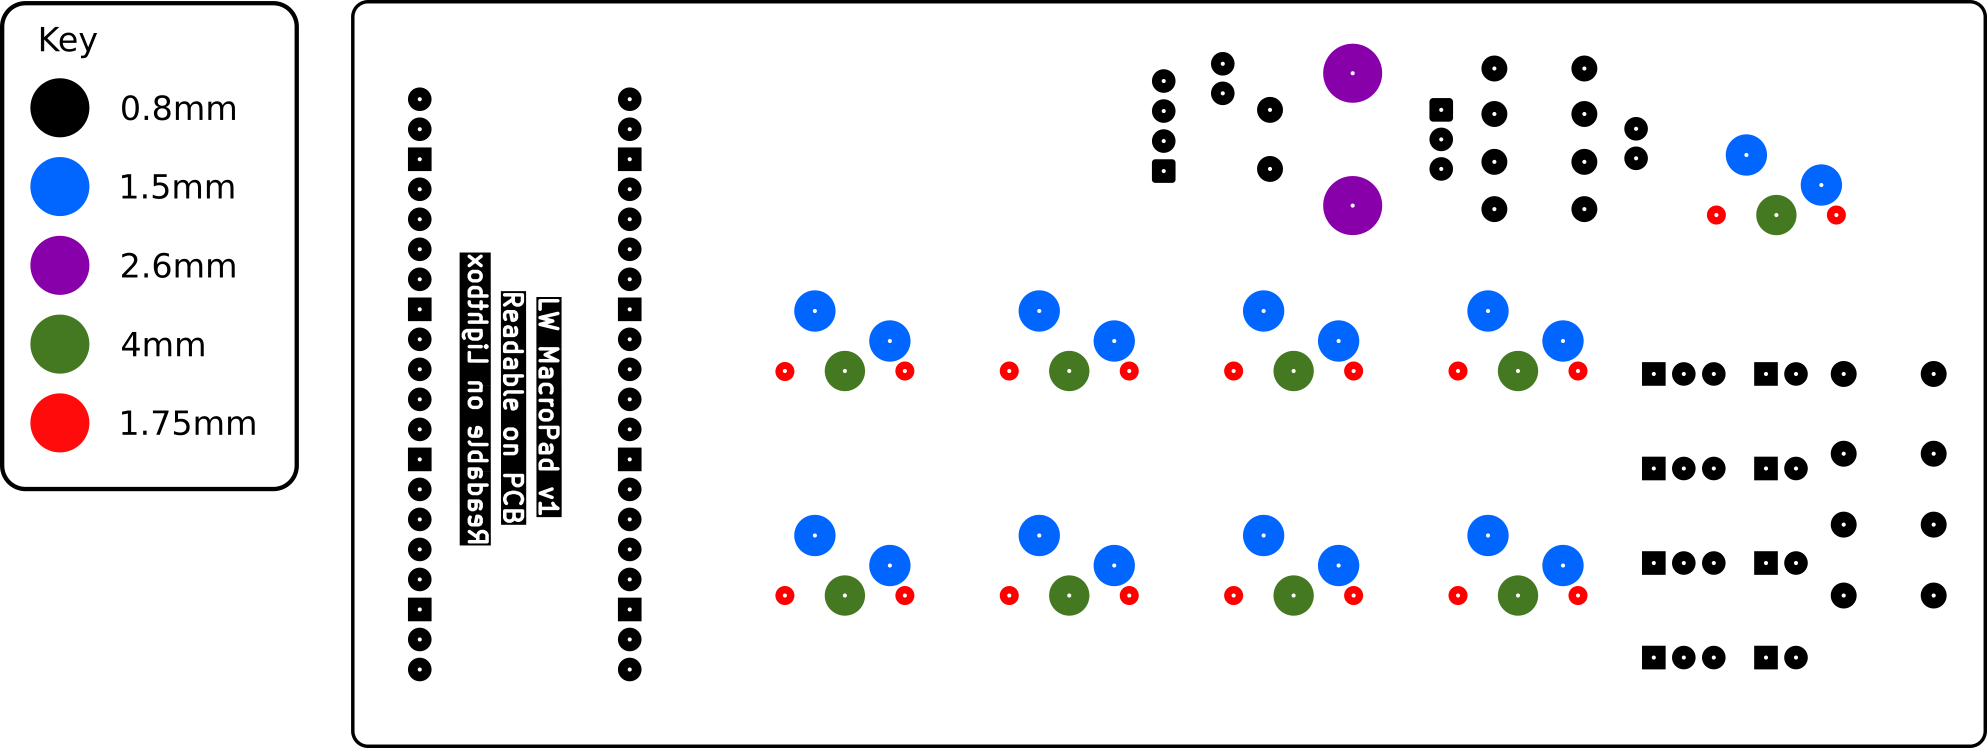
\includegraphics[width=\textheight,angle=90]{img/hole-colours.png}


\section{Parts List}
\label{sec:partslist}

\def\arraystretch{2.5}
\begin{tabular}{cccc}
\hline
\textbf{Reference} & \textbf{Value}        & \textbf{Qty} & \textbf{Order Code}  \\ \hline
C1 - C2            & 10nF                  & 2            &                      \\ \hline
D1 - D4            & LED                   & 4            & WP7113ID             \\ \hline
Q1 - Q4            & 2N7000                & 4            & 2N7000               \\ \hline
R1 - R4            & \ohm{220}             & 4            &                      \\ \hline
R5 - R8            & \ohm{10k}             & 4            &                      \\ \hline
SW1 - SW9          & $\sim$                & 9            & Blue switch          \\ \hline
SW10               & RotaryEncoder\_Switch & 1            & PEC12R-4215F-S0024   \\ \hline
U1                 & Pico                  & 1            & Pi Pico              \\ \hline
U2                 & MDOB128032GV-WI       & 1            & MDOB128032GV-WI      \\ \hline
                   & 4-pin socket          & 1            & 61300411821          \\ \hline
                   & 20-pin header         & 2            & PH1-20-UA            \\ \hline
                   & Key cap               & 9            & -                    \\ \hline
                   & Rotary knob           & 1            & K70105               \\ \hline
                   & Rubber feet           & 5            & SJ5382-TRANSP        \\ \hline
\end{tabular}




\end{document}
